%% Electronic Supplementary Material for the KAIS submission.
%%
%% GENERATED FILE -- do not edit by hand. Generator: scripts/make_kais_main.py
%%
%% Self-contained by design: Springer asks that supplementary captions be
%% intelligible without the main text, so each float below restates what it
%% shows. Floats are lifted verbatim from paper-kbs/kbs-article.tex, so every
%% number matches the artefact-validated source.
\documentclass[11pt,a4paper]{article}
\usepackage[margin=25mm]{geometry}
\usepackage{amsmath}
\usepackage{amssymb}
\usepackage{amsthm}
\usepackage{graphicx}
\usepackage{multirow}
\usepackage{array}
\usepackage{tabularx}
\usepackage{booktabs}
\usepackage{algorithm}
\usepackage{algpseudocode}
\usepackage{microtype}
\usepackage{xurl}
\usepackage{tikz}
\usetikzlibrary{arrows.meta,positioning,fit,backgrounds,calc,shapes.geometric}
\graphicspath{{figures/}}

\hypersetup{hypertexnames=false,bookmarksdepth=3}

%% Figure 1 renders as live TikZ. Set \tikzfigurefalse to fall back to the
%% pre-rendered raster in figures/Fig1.png if the submission system's TeX
%% installation misbehaves with TikZ. This \newif MUST precede the figure:
%% without it \iftikzfigure is an undefined control sequence and the compile
%% dies inside the float.
\newif\iftikzfigure
\tikzfiguretrue

%% Figure lettering. sn-jnl.cls redefines the relative size macros (\tiny is
%% 5pt, \footnotesize is 7pt), both below Springer's 8-12pt floor for figure
%% text, so explicit sizes are set here.
\newcommand{\snFigMain}{\fontsize{9}{10.5}\selectfont}
\newcommand{\snFigSub}{\fontsize{8}{9.5}\selectfont}

\tikzset{
  snstage/.style={
    rectangle, draw=black, line width=0.65pt, fill=white,
    minimum height=18mm, inner sep=3pt, align=center,
    font=\snFigMain, text width=27mm},
  snstagekey/.style={
    rectangle, draw=black, line width=1.0pt, fill=white,
    minimum height=18mm, inner sep=3pt, align=center,
    font=\snFigMain, text width=27mm},
  snfold/.style={
    rectangle, draw=black, dashed, line width=0.5pt, fill=white,
    inner sep=2pt, align=center, font=\snFigSub, text width=19mm},
  snflow/.style={-{Stealth[length=4.5pt,width=3.5pt]}, draw=black,
    line width=0.75pt},
  sndata/.style={-{Stealth[length=4.5pt,width=3.5pt]}, draw=black,
    line width=0.5pt, dashed},
  snout/.style={
    rectangle, draw=black, line width=0.65pt, fill=white,
    minimum height=14mm, inner sep=3pt, align=center,
    font=\snFigMain, text width=34mm},
  sncredit/.style={snout},
  snremoval/.style={snout},
  sninteraction/.style={snout},
  snbranch/.style={draw=black, line width=0.65pt},
  snlbl/.style={font=\snFigSub, inner sep=1.2pt, text=black},
}

\renewcommand{\topfraction}{0.9}
\renewcommand{\bottomfraction}{0.8}
\renewcommand{\textfraction}{0.07}
\renewcommand{\floatpagefraction}{0.6}
\setcounter{topnumber}{3}
\setcounter{bottomnumber}{2}
\setcounter{totalnumber}{5}
\usepackage[section]{placeins}

\theoremstyle{plain}
\newtheorem{theorem}{Theorem}
\newtheorem{proposition}[theorem]{Proposition}
\newtheorem{lemma}[theorem]{Lemma}

\theoremstyle{definition}
\newtheorem{property}{Property}
\newtheorem{remark}{Remark}

\raggedbottom
\emergencystretch=0.75em

\newcommand{\G}{\mathcal{G}}
\newcommand{\Cu}{C_u}
\newcommand{\Ueval}{\mathcal{U}_{\mathrm{eval}}}
\newcommand{\NDCG}{\mathrm{NDCG@10}}
\newcommand{\NDCGat}[1]{\mathrm{NDCG@}#1}
\newcommand{\LOOr}{\mathrm{LOO}_{\mathrm{rank}}}
\newcommand{\LOOe}{\mathrm{LOO}_{\mathrm{e2e}}}
\newcommand{\LOO}{\mathrm{LOO}}

\usepackage{hyperref}

%% S-numbering for every float and section.
\renewcommand{\thesection}{S\arabic{section}}
\renewcommand{\thetable}{S\arabic{table}}
\renewcommand{\thefigure}{S\arabic{figure}}
\renewcommand{\theequation}{S\arabic{equation}}

\title{Electronic Supplementary Material\\[2mm]
\large Ranking-stage source attribution is not source removal:\\
exact Shapley analysis of five-source hybrid recommenders}
\author{Mouad Louhichi \and Redwane Nesmaoui \and Mohamed Lazaar}
\date{}

\begin{document}
\maketitle

\noindent This supplement holds the proofs, the full experimental
configuration, and the robustness suite for the main article. Sections are
numbered S1--S5 and are referenced from the main text. Every table and figure
here is reproduced from the same artefacts as the main article; captions are
written to be read independently.

\tableofcontents
\newpage


\section{Redundancy requires monotonicity}\label{esm:proofs}

The main text states that a natural redundancy property is false without
monotonicity. We record the property, the counterexample, and the corrected
statement here.

\paragraph{The property as usually stated}
If a source is duplicated into the system, one might expect each copy to
receive non-negative credit. This is false for general characteristic
functions.

\paragraph{Counterexample}
Take three players $\{a, b, c\}$ where $b$ and $c$ are exact duplicates, and
let $v$ be non-monotone: $v(\{a\}) = 1$, $v(\{a,b\}) = v(\{a,c\}) = 0.5$,
$v(\{b\}) = v(\{c\}) = v(\{b,c\}) = 0$, $v(\{a,b,c\}) = 0.5$. The duplicated
pair is symmetric, so $\varphi_b = \varphi_c$ by the symmetry axiom, and
efficiency gives $\varphi_a + 2\varphi_b = 0.5$. Direct enumeration yields
$\varphi_b = \varphi_c = -1/12 < 0$. Both copies receive negative credit.

\paragraph{Corrected statement}
If $v$ is monotone, that is $v(S) \le v(T)$ whenever $S \subseteq T$, then
every marginal contribution is non-negative and hence $\varphi_g \ge 0$ for all
$g$, including duplicated players. Monotonicity is the missing hypothesis.

\paragraph{Why this matters empirically}
All three fitted games in the main article are non-monotone
(Table~2 of the main text records the material violation counts), so the
property does not apply to our data. Negative Shapley values in the main
results are therefore faithful computations under a non-monotone game, not
implementation faults. The harmful analytic game in
Table~\ref{tab:analytic} confirms that the implementation recovers a negative
value exactly when one is correct.


\section{Notation and full configuration}\label{esm:config}

Table~\ref{tab:notation} fixes notation. Table~\ref{tab:hyper} gives the
complete experimental configuration, including every hyperparameter, its
value, and how it was selected. Table~\ref{tab:provenance} maps each group of
reported results to the artefact, platform, candidate rule and seed range that
produced it, including the one group that was regenerated under a different
candidate rule.

\begin{table}[htbp]
\caption{Core notation.}
\label{tab:notation}
\centering
\small
\begin{tabularx}{\columnwidth}{@{}lX@{}}
\toprule
Symbol & Meaning \\
\midrule
$\G$ & five source players \\
$\mathcal{U},\Ueval$ & retained users and users with nonempty candidates \\
$\Cu,\Cu(S)$ & fixed and coalition-specific candidate sets \\
$Z_u^{(S)},w^{(S)}$ & standardized source scores and coalition head \\
$b_u$ & expected NDCG@10 of a random ranking of $\Cu$ \\
$v_u(S),v(S)$ & per-user and mean baseline-centred utilities \\
$\varphi_g,\varphi_g(u)$ & Shapley value of source $g$, and its per-user term \\
$\LOOr,\LOOe$ & ranking-stage and end-to-end leave-one-out \\
$\rho$ & retrievability ceiling: fraction of $\Ueval$ whose test item is
         not masked by training history \\
$\lambda$ & ridge penalty of the coalition head (summed loss) \\
$\lambda_{\mathrm{ALS}}$ & regularisation of the $cf$ ALS factorisation \\
$\gamma_{\mathrm{shrink}}$ & shrinkage of segment fusion weights toward the
         global profile (this section of the main article) \\
\bottomrule
\end{tabularx}
\end{table}
\begin{table}[htbp]
\caption{Experimental configuration.}
\label{tab:hyper}
\footnotesize
\setlength{\tabcolsep}{3pt}
\begin{tabularx}{\textwidth}{@{}ll>{\raggedright\arraybackslash}p{0.26\textwidth}X@{}}
\toprule
Component & Parameter & Value & Note \\
\midrule
$cf$  & latent factors        & $64$    & ALS, implicit feedback \\
      & confidence scaling    & $\alpha = 1$, $c_{ui} = 1 + \alpha r_{ui}$ & binarised $r_{ui}$ \\
      & regularisation        & $0.1$   & \\
      & alternating iterations& $15$    & \\
$ct$  & TF--IDF vocabulary    & $5000$  & token pattern \texttt{\textbackslash S+} \\
$pop$ & decay half-life       & $180$ d & exponential \\
$rec$ & content clusters      & $20$    & argmax over a $20$-component truncated
                                            SVD of a separate $2\,000$-vocabulary
                                            TF--IDF item matrix (no $k$-means);
                                            \texttt{random\_state} $=$ seed \\
      & TF--IDF vocabulary      & $2000$  & separate from $ct$'s $5000$ \\
      & decay half-life       & $30$ d  & \\
$seq$ & embedding dimension   & $64$    & PPMI--SVD \\
      & PPMI shift            & $k_{\mathrm{s}} = 1$, so $\log k_{\mathrm{s}} = 0$ & unshifted: the configuration is plain PPMI--SVD \\
      & co-occurrence window  & $5$     & \\
\midrule
Game  & $N_{\max}$            & $600$ / $600$ / $11\,623$ & ML-1M / Amazon-VG / Gowalla \\
      & ridge $\lambda$       & $1.0^{\dagger}$ & summed-loss parameter. The
        comparable averaged-loss value $\lambda/|\mathcal U_{\rm fit}|$ is
        $1.66\times10^{-4}$, $1.40\times10^{-4}$ and $1.13\times10^{-4}$ for
        ML-1M, Amazon-VG and Gowalla, so $\lambda=1$ is not the same
        effective penalty across corpora \\
      & NDCG cutoff $K$       & $10$    & \\
      & empty-coalition baseline & $\mathbb{E}[\NDCG]$ & Equation~(the characteristic function of the main article); deterministic, no seed \\
      & ranking tie rule      & score, then item index & exact total order; no tolerance relation \\
      & initial per-source depth & $\lceil N_{\max}/n \rceil$ & $120$ for $N_{\max}=600$, equal for every source \\
      & candidate growth iters& $10$    & $N_g \gets N_g + \lceil (N_{\max} - |C_u|)/n \rceil$ per pass \\
      & recall gate           & $0.60$  & see the preconditions of the main article \\
      & materiality threshold & $10^{-3}$ & reporting only, not a theorem \\
\midrule
Fusion& segments             & $4$     & activity $\times$ recency, median splits \\
      & softmax $\tau$        & $\{0.001, 0.01, 0.1\}^{\dagger}$ & validation-selected \\
      & shrinkage $\gamma_{\mathrm{shrink}}$ & $\{0, 0.5, 1\}^{\dagger}$ & validation-selected \\
\midrule
LightGCN & factors / layers   & $64$ / $3$ & contextual reference only \\
      & epochs / lr / reg     & $40$ / $0.01$ / $10^{-4}$ & \\
SASRec& dim / max length      & $64$ / $50$ & contextual reference only \\
      & blocks / epochs / lr  & $2$ / $25$ / $0.05$ & \\
\midrule
Protocol & seeds              & $42$--$51$ (run-to-run summaries) & seed $42$ alone for labelled single-run diagnostics \\
      & source random state   & seed & passed to ALS and every truncated SVD \\
      & split                 & leave-last-out & test $=$ last, validation $=$ second-last \\
      & tie-break             & (timestamp, record index) & \\
\bottomrule
\end{tabularx}
\smallskip
\noindent\footnotesize $^{\dagger}$Selected on a MovieLens pilot and then
frozen. All other values are prespecified implementation settings and were not
tuned separately by corpus or coalition; $N_{\max}$ alone varies by corpus.
\end{table}
\begin{table}[htbp]
\caption{Provenance of reported result groups.}
\label{tab:provenance}
\centering
\small
\begin{tabular}{@{}p{0.30\textwidth}p{0.10\textwidth}p{0.32\textwidth}p{0.16\textwidth}@{}}
\toprule
Result & Seeds & Candidate rule & Role \\
\midrule
Attribution and retirement & 42--51 & source-symmetric & primary \\
Pairwise interactions & 42--51 & source-symmetric & explanatory \\
Neutral candidate pools & 42 & all four pool rules & sensitivity \\
Semivalues and interactions & 42 & source-symmetric (ML-1M, Gowalla);
  legacy (Amazon-VG) & sensitivity \\
Estimand comparison (Table~\ref{tab:estimands}) & 42 & refitted head
  source-symmetric; fixed head and end-to-end legacy & sensitivity \\
Globally blocked replication & 42 & source-symmetric & stress test \\
Preconditions and duplicate test & 42--44 & source-symmetric$^{\ast}$ & sensitivity \\
Sweeps, ablations, and segments & 42--44 & source-symmetric$^{\ast}$ & exploratory \\
\bottomrule
\end{tabular}
\smallskip
\noindent\footnotesize $^{\ast}$MovieLens-1M and Amazon-VG only. The Gowalla
diagnostics remain under the legacy rule: regenerating them requires holding
five dense $8\,865 \times 82\,134$ score matrices, which exhausted memory on
the $48$\,GB machine used for these runs. Gowalla's primary attribution and
retirement numbers are unaffected, since those come from the ten-seed
artefact, which is source-symmetric on all three corpora.
\end{table}

\section{Verification detail and the robustness suite}\label{esm:robustness}

\subsection{Analytic games and duplicate injection}

Table~\ref{tab:analytic} lists the six analytic games with known Shapley
vectors and the maximum absolute recovery error on each, which is zero
throughout. Table~\ref{tab:recovery} reports the duplicate-injection
diagnostics on MovieLens-1M: an exact clone of the collaborative source
receives credit equal to its original to numerical precision, while
leave-one-out assigns both clones zero.

\subsection{Alternative values and interactions}

Table~\ref{tab:taylor} gives the pairwise Shapley interaction indices on
MovieLens-1M over ten stochastic fits. The two most negative pairs,
$cf$--$seq$ and $cf$--$pop$, are the substitutions declared in advance in the
main text, so the declared overlap is partially recovered by the data.

Semivalue comparison, summarised in the main text, is as follows.
On MovieLens-1M, Banzhaf and both binomial semivalues rank the five sources
identically to Shapley. The size-uniform semivalue is algebraically identical
to Shapley, since
$|S|!\,(n-|S|-1)!/n! = 1/\bigl(n\binom{n-1}{|S|}\bigr)$, and agrees to exactly
zero difference; we note this because the identity is easy to miss and makes
that particular comparison vacuous. On Gowalla, Banzhaf and both binomial
semivalues agree with Shapley at $\tau = 0.80$; the $q = 0.25$ semivalue
promotes $ct$ over $cf$ across a margin of $0.00037$, and Banzhaf and
$q = 0.75$ transpose $pop$ and $rec$ across a margin of $0.00017$. On
Amazon-VG the disagreement is stronger and we report it as a limitation of the
robustness claim: $\tau = 0.60$, with Shapley leading on $cf$ and Banzhaf on
$seq$.

\subsection{Sensitivity analyses}

Table~\ref{tab:ablations} summarises the ablation and sensitivity suite.
Figure~\ref{fig:robustness} shows the candidate-cap and ridge-penalty sweeps at
seed 42, and Figure~\ref{fig:redundancy} the pairwise source-score rank
correlations by corpus. Figure~\ref{fig:shares} gives per-source Shapley values
with seed-based intervals on all three corpora.

The headline robustness results, each verified against its artefact, are:
the ridge penalty $\lambda$ swept over eight orders of magnitude leaves both
material sign flips intact; three source-blind candidate pool rules leave both
flips intact, and oracle-pool recall equals $\rho$ exactly on every corpus,
which independently confirms the dilution identity; Gaussian score perturbation
at $\sigma \in \{0.1, 0.5\}$ in units of each source's own standard deviation
leaves both flips intact on all three corpora; refreshing the frozen temporal
state raises $v(\G)$ on MovieLens-1M by $31.7\%$ $[+30.2\%, +33.1\%]$ while
preserving the ordering at $\tau = 1.00$ on all ten seeds; and swapping the
payoff metric to Recall@10 or MRR@10 preserves the ordering at $\tau = 1.00$.

ESM~Table~S8 audits repeat events, which is what produces the
retrievability ceiling on Gowalla: $49.90\%$ of evaluated users there have
their test venue already in training, and masking makes it unretrievable, so
those users contribute zero to every coalition.

\subsection{Three estimands}

Table~\ref{tab:estimands} reports the same seed-42 game under three
constructions: the refitted head used in the main text, a fixed grand-coalition
head merely masked to each coalition, and a fully end-to-end game in which each
coalition retrieves its own candidates. The refitted-head rows use the final
source-symmetric candidate rule; the other two predate that regeneration and
are retained as a sensitivity analysis, so the table compares \emph{orderings}
across estimands rather than numerical estimates from a single artefact.

\begin{table}[htbp]
\caption{Exact Shapley recovery on six analytic games.}
\label{tab:analytic}
%% \small and a p{} column: the characteristic functions are long enough
%% that `l' pushed this table past the text block.
\small
\begin{tabular}{@{}lp{0.44\textwidth}cc@{}}
\toprule
Game & Characteristic function $v(S)$ & Expected $\varphi$ & Max error \\
\midrule
Additive     & $\sum_{g\in S} c_g$, \ $c=(3,2,1)$                & $(3, 2, 1)$  & $0$ \\
Substitutes  & $4\cdot\mathbb{1}[\{s_1,s_2\}\cap S \neq \varnothing] + \mathbb{1}[x\in S]$
                                                                  & $(2, 2, 1)$  & $0$ \\
Complements  & $6\cdot\mathbb{1}[\{c_1,c_2\}\subseteq S] + 2\cdot\mathbb{1}[x\in S]$
                                                                  & $(3, 3, 2)$  & $0$ \\
Null player  & $\sum_{g\in S\cap\{a,b\}} c_g$, \ $c=(3,2)$        & $(3, 2, 0)$  & $0$ \\
Harmful      & $5\cdot\mathbb{1}[a\in S] - 2\cdot\mathbb{1}[\mathit{bad}\in S]$
                                                                  & $(5, -2)$    & $0$ \\
Unanimity    & $9\cdot\mathbb{1}[S = \G]$                          & $(3, 3, 3)$  & $0$ \\
\bottomrule
\end{tabular}
\end{table}
\begin{table}[htbp]
\caption{MovieLens-1M duplicate-source diagnostics ($cf$ clone, $\eta=0$).}
\label{tab:recovery}
\begin{tabular}{@{}lrrrrr@{}}
\toprule
Corpus & $\lambda$ & Sym.\ err. & $\Delta_{\mathrm{red}}$ &
$\varphi(cf) = \varphi(cf_{\mathrm{dup}})$ &
$\LOO(cf)$, $\LOO(cf_{\mathrm{dup}})$ \\
\midrule
\multirow{2}{*}{MovieLens-1M} & frozen & $0.0$ & $0.0$ & $0.010781$ & $0.000000$, $0.000000$ \\
                              & $0$    & $0.0$ & $0.0$ & $0.010781$ & $0.000000$, $0.000000$ \\
\bottomrule
\end{tabular}
\end{table}
\begin{table}[htbp]
\caption{MovieLens-1M pairwise Shapley interactions over ten stochastic fits.}
\label{tab:taylor}
\centering
\footnotesize
\setlength{\tabcolsep}{2.5pt}
\begin{tabular}{@{}lrcc@{}}
\toprule
Pair & $\mathcal{I}_{ab}$ (10-seed mean) & run interval & Neg.\ seeds \\
\midrule
$cf$--$seq$  & $-0.0542$ & $[-0.0554, -0.0529]$ & $10/10$ \\
$cf$--$pop$  & $-0.0254$ & $[-0.0256, -0.0252]$ & $10/10$ \\
$ct$--$pop$  & $-0.0027$ & $[-0.0029, -0.0025]$ & $10/10$ \\
$pop$--$rec$ & $-0.0017$ & $[-0.0019, -0.0016]$ & $10/10$ \\
$cf$--$rec$  & $-0.0011$ & $[-0.0014, -0.0009]$ & $10/10$ \\
$rec$--$seq$ & $-0.0011$ & $[-0.0014, -0.0009]$ & $10/10$ \\
$ct$--$rec$  & $+0.0004$ & $[+0.0003, +0.0006]$ & $0/10$ \\
$ct$--$seq$  & $+0.0012$ & $[+0.0009, +0.0014]$ & $0/10$ \\
$cf$--$ct$   & $+0.0020$ & $[+0.0016, +0.0023]$ & $0/10$ \\
$pop$--$seq$ & $+0.0059$ & $[+0.0056, +0.0061]$ & $0/10$ \\
\bottomrule
\end{tabular}
\end{table}
\begin{table}[htbp]
\caption{Ablation and sensitivity summary.}
\label{tab:ablations}
\small
\begin{tabularx}{\textwidth}{@{}p{0.25\textwidth}p{0.20\textwidth}X@{}}
\toprule
Design contrast & Scope & Main outcome \\
\midrule
Union vs grand-coalition pool & MovieLens, seed 42 & Recall $0.748\to0.807$;
$\varphi_{ct}$ changes sign (the cooperative game of the main article). \\
Symmetric vs source-ordered truncation & MovieLens probe & Maximum attribution
change $2.8\times10^{-5}$; ordering unchanged (the cooperative game of the main article). \\
Retain vs drop validation misses & Three corpora, seed 42 & All signs unchanged;
maximum shift $2.1\times10^{-4}$ (the algorithm of the main article). \\
Frozen vs refreshed history & Three corpora, seed 42 & $v(\G)$ changes by
$36\%$, $19\%$, and $3.7\%$; ordering changes on Amazon-VG
(the algorithm of the main article). \\
Ridge-penalty sweep & Three corpora, seed 42 & The two material sign
disagreements persist over $10^{-5}$--$10^3$ (the results of the main article). \\
Gowalla user subsample & Ten seeds & Signs persist; source-order agreement is
$\tau=0.80$ (the results of the main article). \\
\bottomrule
\end{tabularx}
\end{table}
\begin{table}[htbp]
\caption{Repeat-event audit; masked test items yield zero payoff for every
coalition.}
\label{tab:repeats}
\small
\begin{tabular}{@{}lrrrr@{}}
\toprule
Corpus & Users & Val.\ $=$ test item & Test item in train & Repeat events \\
\midrule
MovieLens-1M & 6\,035 & $0$ ($0.00\%$)    & $0$ ($0.00\%$)      & $0.00\%$ \\
Amazon-VG    & 7\,120 & $430$ ($6.04\%$)  & $198$ ($2.78\%$)    & $5.27\%$ \\
Gowalla      & 8\,865 & $1\,260$ ($14.21\%$) & $4\,424$ ($49.90\%$) & $52.61\%$ \\
\bottomrule
\end{tabular}
\end{table}
\begin{table}[htbp]
\caption{Three attribution games at seed 42; $\tau$ is Kendall
agreement with the refitted-head game.}
\label{tab:estimands}
\small
\setlength{\tabcolsep}{3.5pt}
\begin{tabular}{@{}llrrrrrc@{}}
\toprule
Corpus & Game & $cf$ & $ct$ & $pop$ & $rec$ & $seq$ & $\tau$ \\
\midrule
MovieLens-1M & refitted head$^{\ast}$ & $+0.01545$ & $-0.00009$ & $+0.00637$ & $+0.00026$ & $+0.02937$ & n/a \\
             & fixed head$^{\dagger}$  & $+0.01867$ & $-0.00104$ & $+0.00528$ & $-0.00079$ & $+0.02924$ & $1.00$ \\
             & end-to-end$^{\dagger}$  & $+0.01478$ & $-0.00010$ & $+0.00783$ & $-0.00022$ & $+0.02908$ & $0.80$ \\
\midrule
Amazon-VG    & refitted head$^{\ast}$ & $+0.01926$ & $+0.00187$ & $+0.00157$ & $-0.00047$ & $+0.01909$ & n/a \\
             & fixed head$^{\dagger}$  & $+0.02110$ & $+0.00101$ & $+0.00166$ & $-0.00045$ & $+0.01799$ & $0.80$ \\
             & end-to-end$^{\dagger}$  & $+0.01962$ & $+0.00133$ & $+0.00291$ & $+0.00026$ & $+0.01718$ & $0.80$ \\
\bottomrule
\end{tabular}
\par\smallskip
\begin{minipage}{0.92\textwidth}
\raggedright\footnotesize
$^{\ast}$Final source-symmetric candidate rule; these are the seed-42 main
results used elsewhere in the paper. $^{\dagger}$Legacy candidate rule,
retained as a sensitivity analysis only: these rows predate the truncation-key
regeneration and are not artefact-matched to the refitted-head row. The table
compares \emph{orderings} across estimands rather than numerical estimates
drawn from one artefact.
\end{minipage}
\end{table}
\begin{figure}[htbp]
\centering
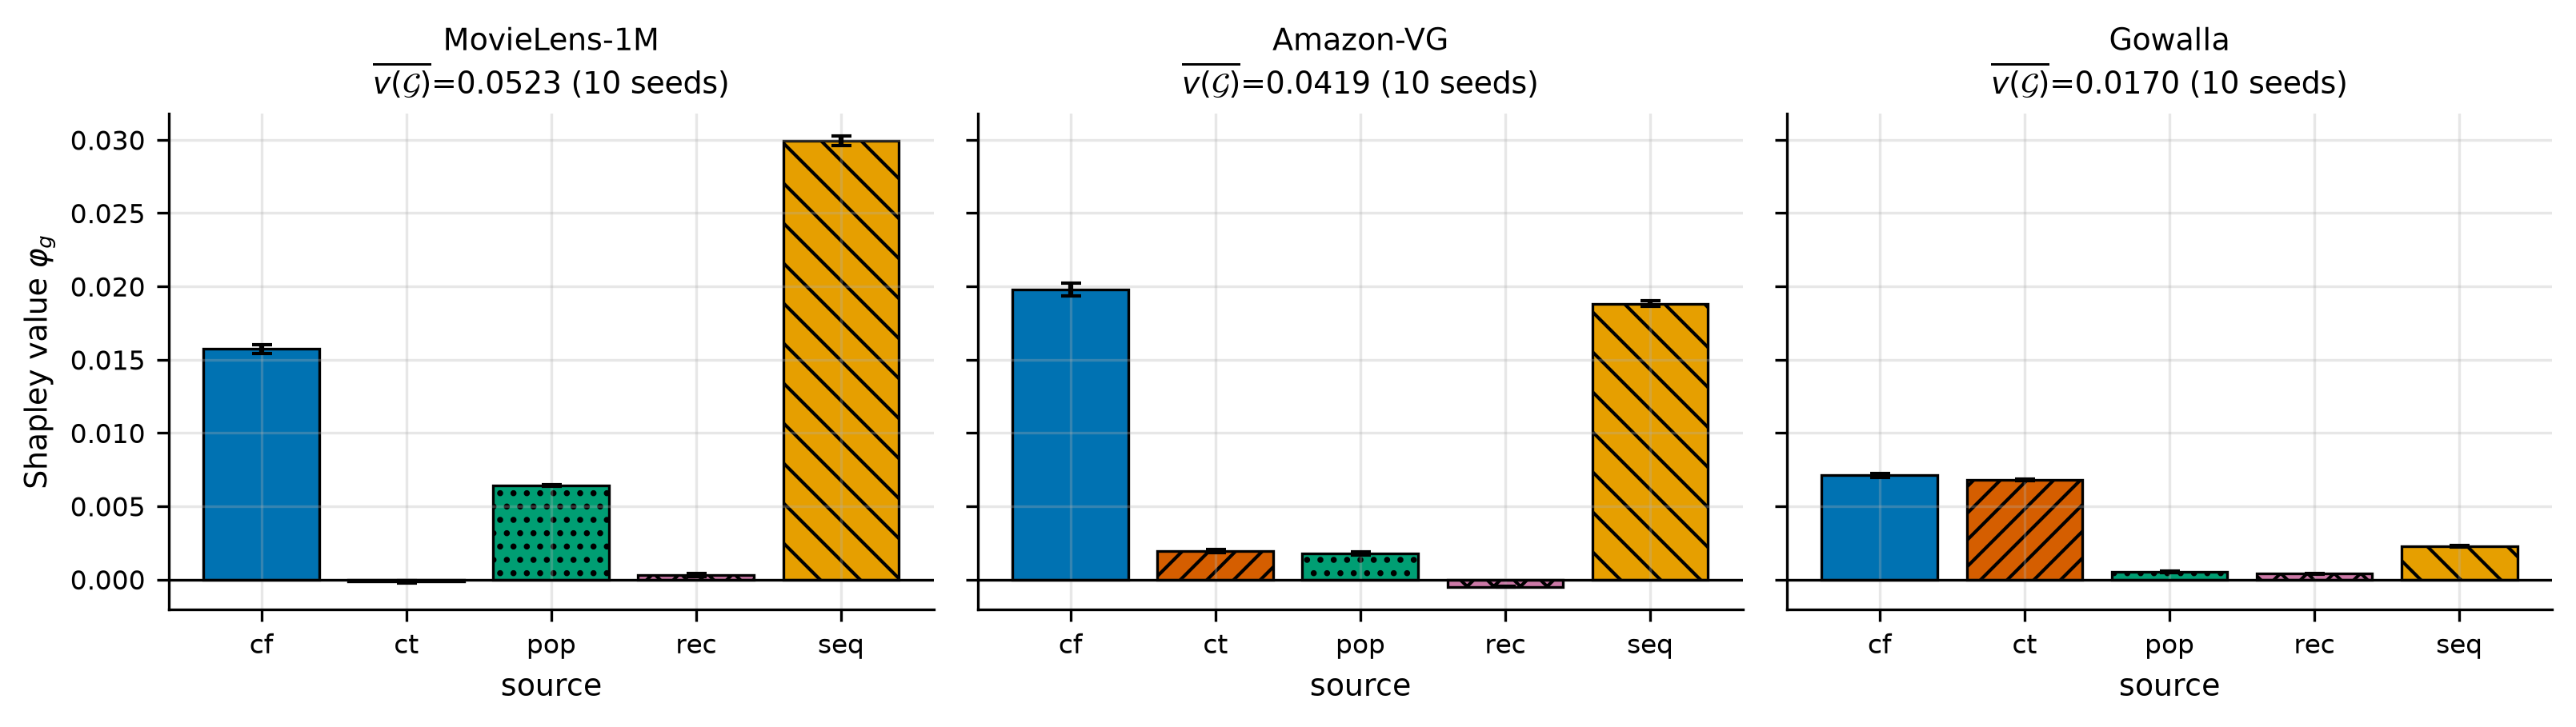
\includegraphics[width=\textwidth]{Fig2.png}
\caption{Per-source Shapley values over seeds 42--51; whiskers show
$\bar{x}\pm t_9\mathrm{SE}$.}
\label{fig:shares}
\end{figure}
\begin{figure}[htbp]
\centering
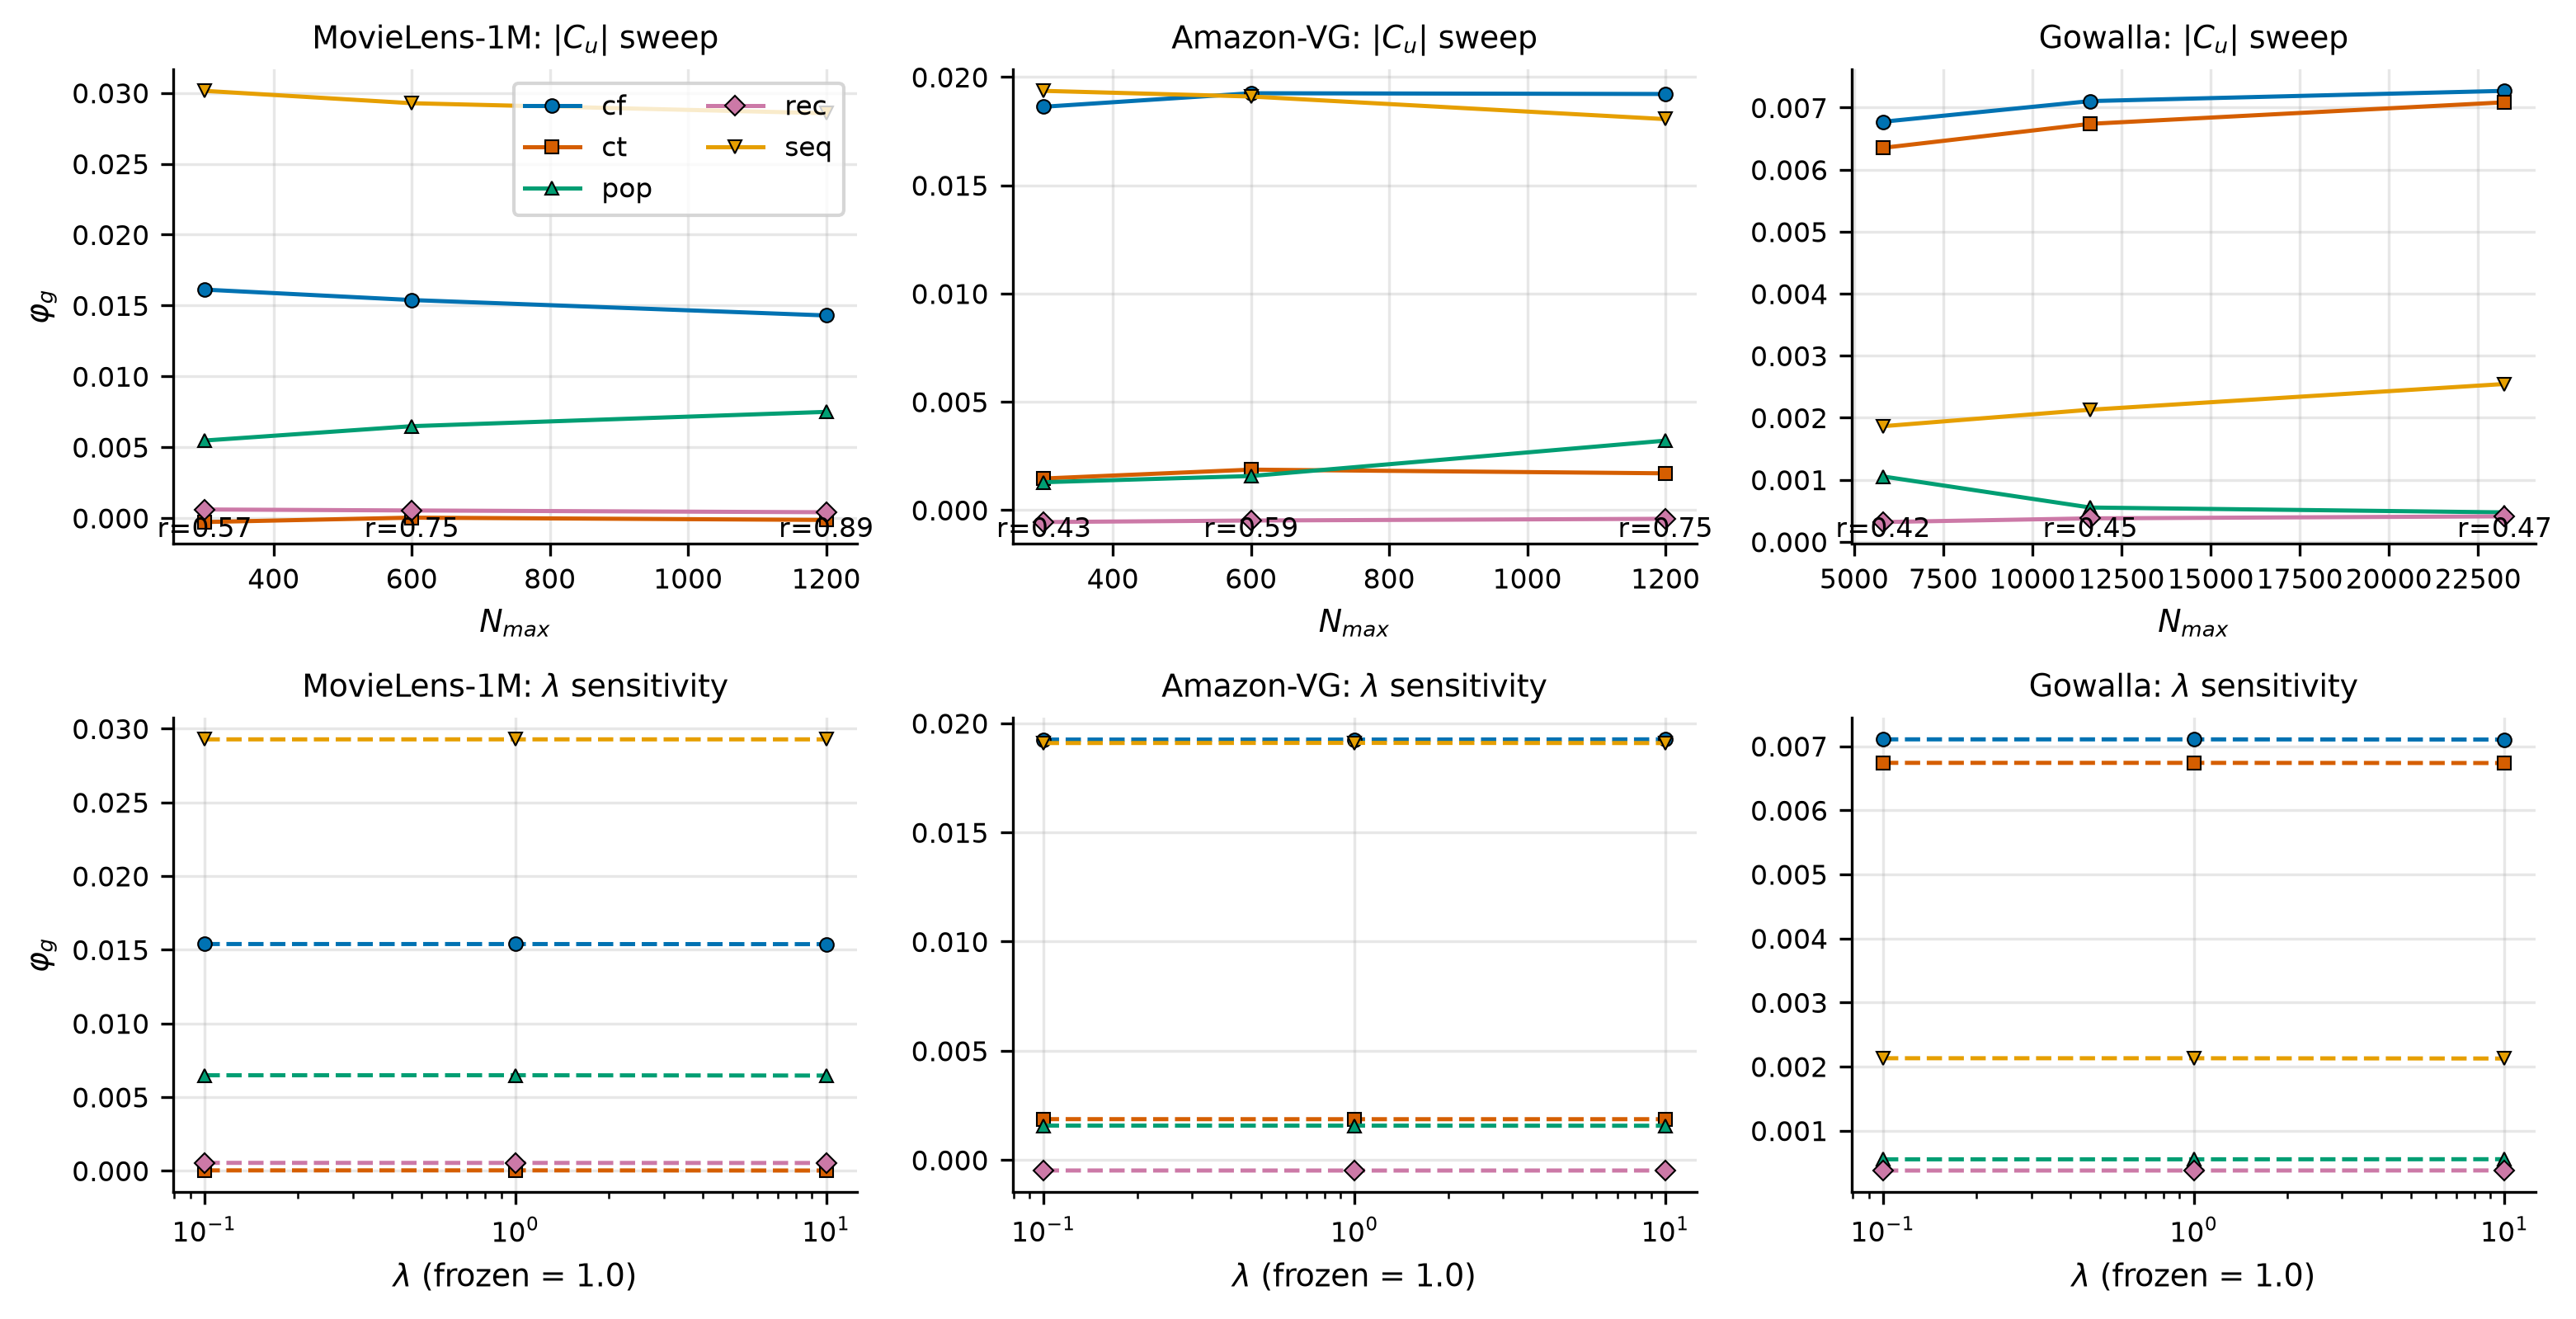
\includegraphics[width=\textwidth]{Fig7.png}
\caption{Candidate-cap and ridge-penalty sensitivity at seed 42; labels show
candidate recall.}
\label{fig:robustness}
\end{figure}
\begin{figure}[htbp]
\centering
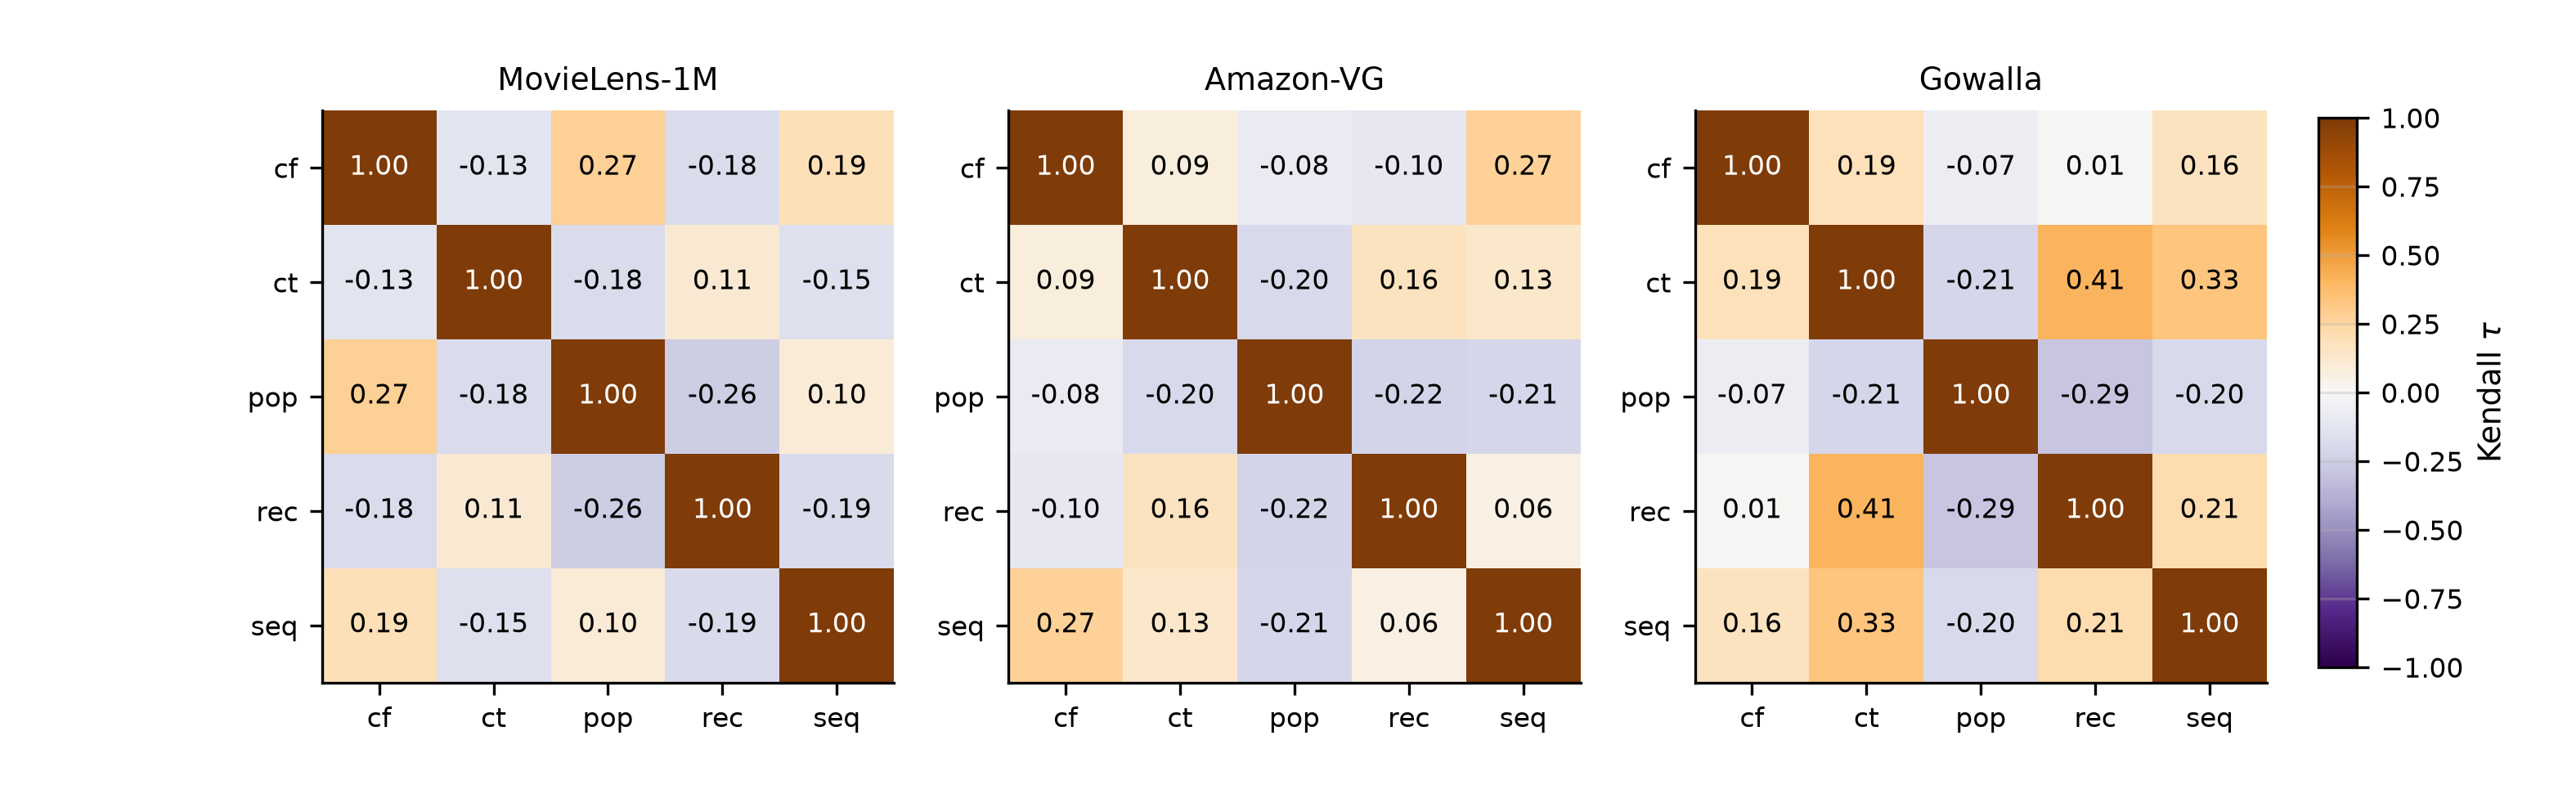
\includegraphics[width=\textwidth]{Fig4.png}
\caption{Pairwise source-score Kendall $\tau$ by corpus.}
\label{fig:redundancy}
\end{figure}

\section{Sampling error against exact enumeration}\label{esm:sampling}

The main text reports that permutation sampling at $M = 500$ has a
95th-percentile error exceeding both the ten-seed spread and the materiality
threshold. Table~\ref{tab:sampling-esm} gives the full grid behind
Figure~8 of the main article.

\begin{table}[htbp]
\centering
\caption{Sampled Shapley error against exact enumeration on a complete
32-coalition game, over 20 repeats per budget. Values are
$\|\hat\varphi - \varphi\|_\infty$ as a percentage of $v(\G)$. For reference,
the ten-seed spread of the fitted values is $2.22\%$ and the $10^{-3}$
materiality threshold is $1.91\%$ of $v(\G)$.}
\label{tab:sampling-esm}
\small
\begin{tabular}{@{}lrrrr@{}}
\toprule
& \multicolumn{2}{c}{Permutation sampling} & \multicolumn{2}{c}{KernelSHAP} \\
\cmidrule(lr){2-3}\cmidrule(lr){4-5}
Budget $M$ & Mean & p95 & Mean & p95 \\
\midrule
$50$   & $6.68\%$ & $10.84\%$ & $20.85\%$ & $25.93\%$ \\
$100$  & $3.32\%$ & $6.33\%$  & $11.44\%$ & $18.60\%$ \\
$500$  & $1.62\%$ & $2.73\%$  & $4.87\%$  & $9.88\%$ \\
$2000$ & $0.90\%$ & $2.16\%$  & $2.34\%$  & $3.67\%$ \\
\bottomrule
\end{tabular}
\end{table}

The measurement uses the end-to-end recall game, which is the only complete
32-coalition characteristic function persisted in the released artefacts.
Enumeration on it satisfies efficiency to $1.1\times10^{-16}$, confirming the
estimator harness. Absolute errors do not transfer to the NDCG@10 game of the
main text; errors relative to $v(\G)$ do, which is why the table is expressed
that way. KernelSHAP is the weaker estimator here because at $n = 5$ its kernel
concentrates on few coalition sizes.


\section{Full decision-to-estimand mapping}\label{esm:decisions}

The main article gives a five-row summary of which estimand answers which
question. Table~\ref{tab:decisions} is the complete mapping, including the rows
that were compressed for length. It records, for each decision a practitioner
might want to make, the quantity that actually answers it and whether this
study establishes that quantity or leaves it open.

\begin{table}[htbp]
\caption{Decision-to-estimand mapping.}
\label{tab:decisions}
%% p{} columns, not l: the third column carries a sentence and `l' cannot
%% wrap, so the row ran past the text block.
\begin{tabular}{@{}p{0.30\textwidth}p{0.30\textwidth}p{0.32\textwidth}@{}}
\toprule
Decision & Quantity aligned with question & Evidence in this study \\
\midrule
Remove one deployed source
  & $\LOOe$ by definition; $\LOOr$ a measured proxy here
  & $\tau = 0.96$--$1.00$ over 10 seeds (the retirement comparison of the main article) \\[2pt]
Divide baseline-centred ranking utility
  & Shapley under the declared game and axioms
  & efficiency and symmetry checks (the verification section of the main article) \\[2pt]
Rank sources under a different
coalition weighting
  & a declared semivalue (Banzhaf, binomial)
  & ordering agrees on MovieLens (the semivalue comparison of the main article); these do
    \emph{not} sum to $v(\G)$, so they rank rather than divide \\[2pt]
Locate pairwise interaction under the game
  & pairwise interaction index
  & Table~\ref{tab:taylor} \\[2pt]
Decide where to invest next
  & \emph{not established}
  & would need cost and headroom, which $v$ does not contain \\[2pt]
Trust the result under globally
causal chronology
  & the allocation-versus-removal contrast, not the named sources
  & under a global cutoff the per-source attributions do not replicate, while
    $\LOOr$ still leads Shapley ($\tau = 0.80$ against $0.60$) on a population
    retaining $8.7\%$ of users at recall $0.464$
    (the threats to validity of the main article) \\[2pt]
Trust the result when the players
did not build the pool
  & the material disagreements
  & both survive candidate pools that consult no source score; the oracle pool
    returns recall equal to $\rho$ exactly (the threats to validity of the main article) \\
\bottomrule
\end{tabular}
\end{table}

\section{Attribution-derived fusion: a negative result}\label{esm:fusion}

This section reports an experiment that did not work. We include it because the
natural next step after allocating credit is to \emph{use} the allocation, and
a reader is entitled to know that we tried and that it failed.

We mapped Shapley values to fusion weights, both globally and per user segment,
and compared the resulting ranker against the matched global head on the full
catalogue. Attribution-derived fusion gives no resolvable gain. Fusion weights
never see test outcomes, so this is not a leakage artefact; the allocation
simply is not a good weight vector, which is consistent with the main article's
position that the allocation is descriptive rather than prescriptive.

Figure~\ref{fig:fusion} shows the full-catalogue comparison and
Figure~\ref{fig:segments} the descriptive segment-level values. Segment
heterogeneity is descriptive only: segments were not pre-declared and the
comparison is not powered for segment-level inference. No cross-corpus omnibus
ranking is computed, because the corpora differ in protocol and cannot be
pooled.

This appendix is a negative result about one downstream use of the
attributions. It is not evidence for or against their correctness, which rests
on the checks in Section~\ref{esm:robustness}.

\begin{figure}[htbp]
\centering
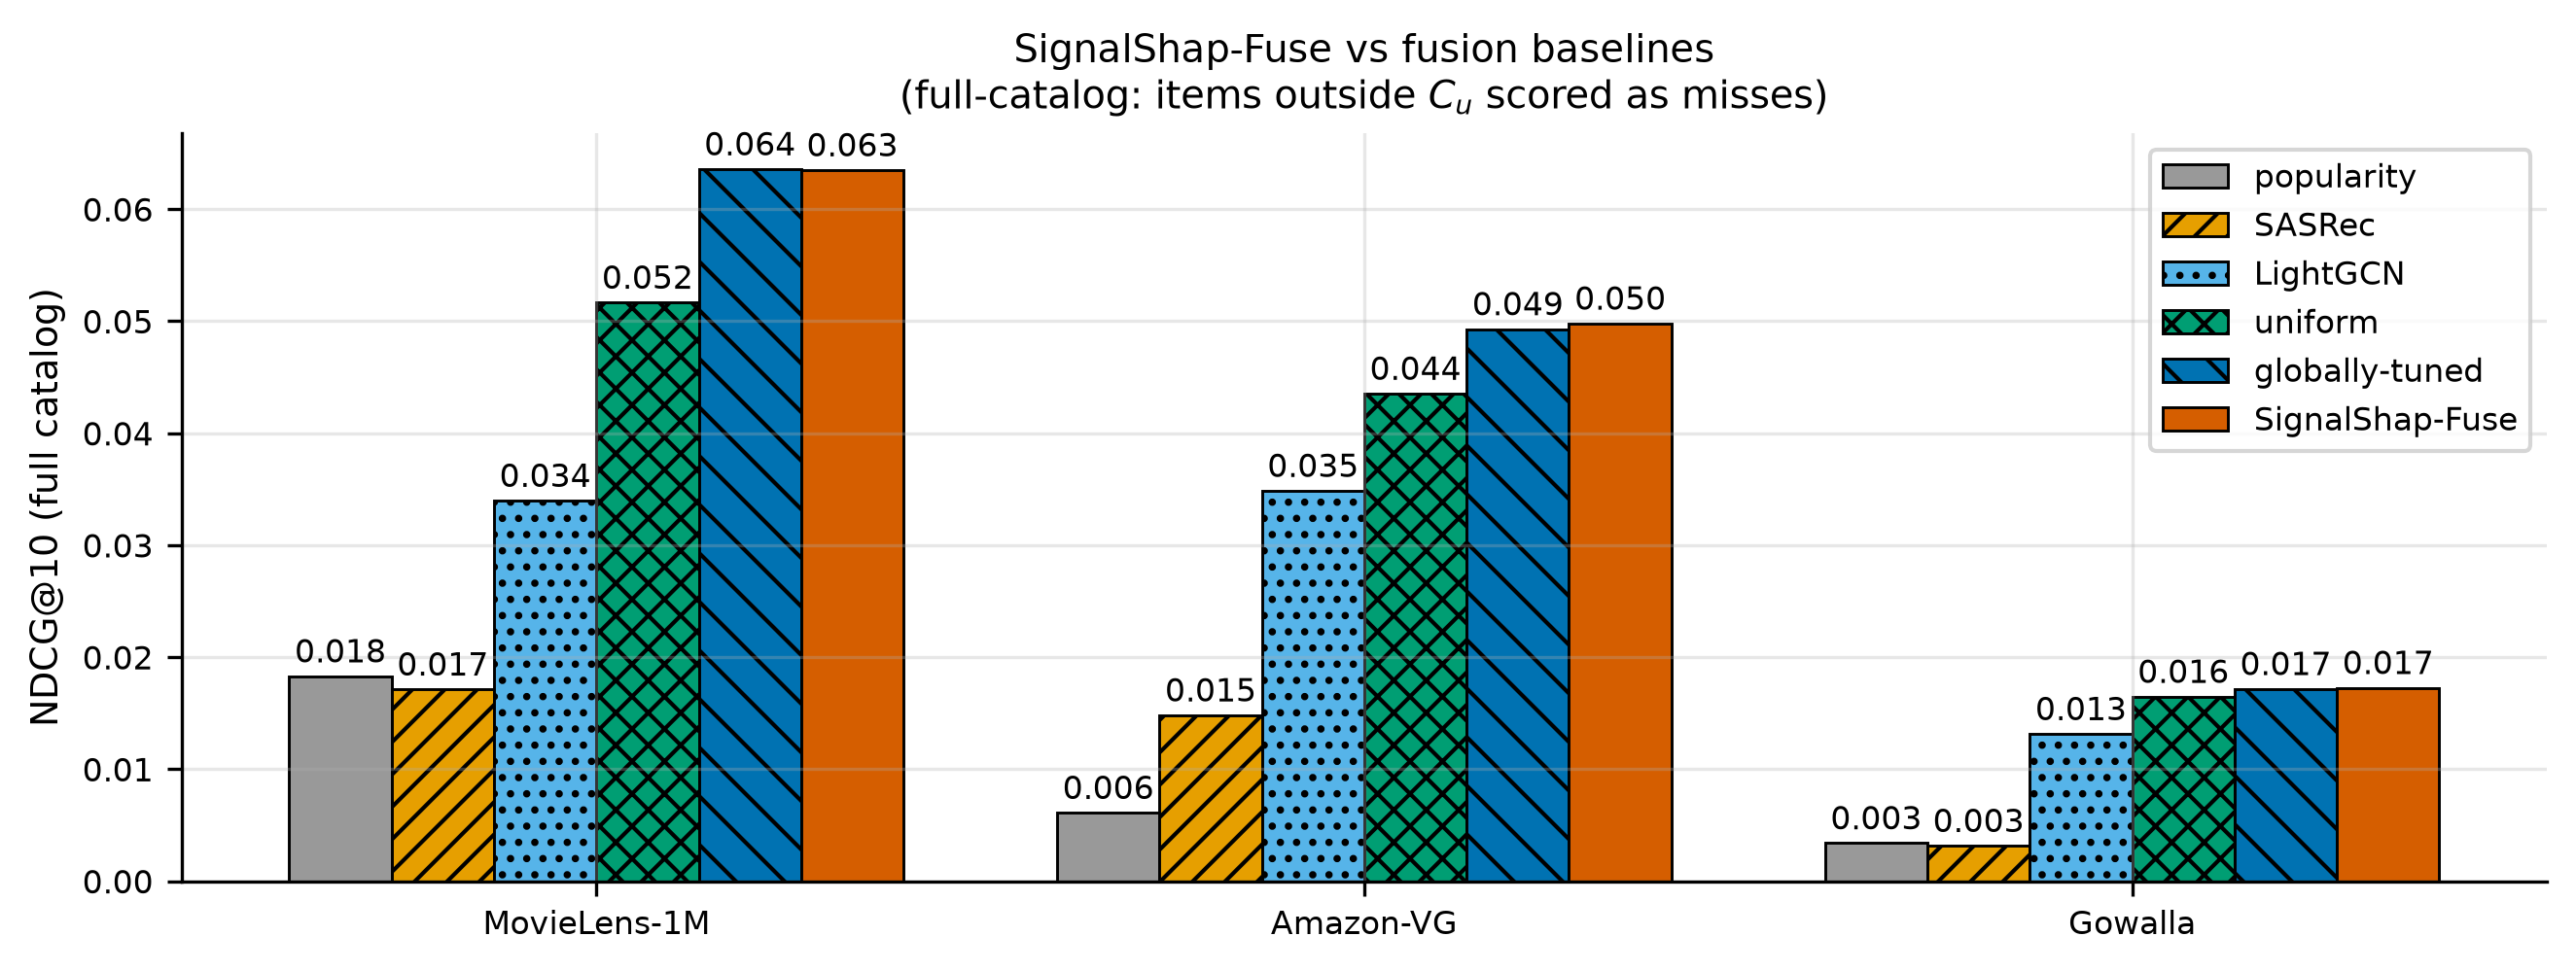
\includegraphics[width=0.85\textwidth]{Fig6.png}
\caption{Full-catalogue fusion comparison; Amazon-VG and Gowalla remain below
the candidate-recall gate.}
\label{fig:fusion}
\end{figure}
\begin{figure}[htbp]
\centering
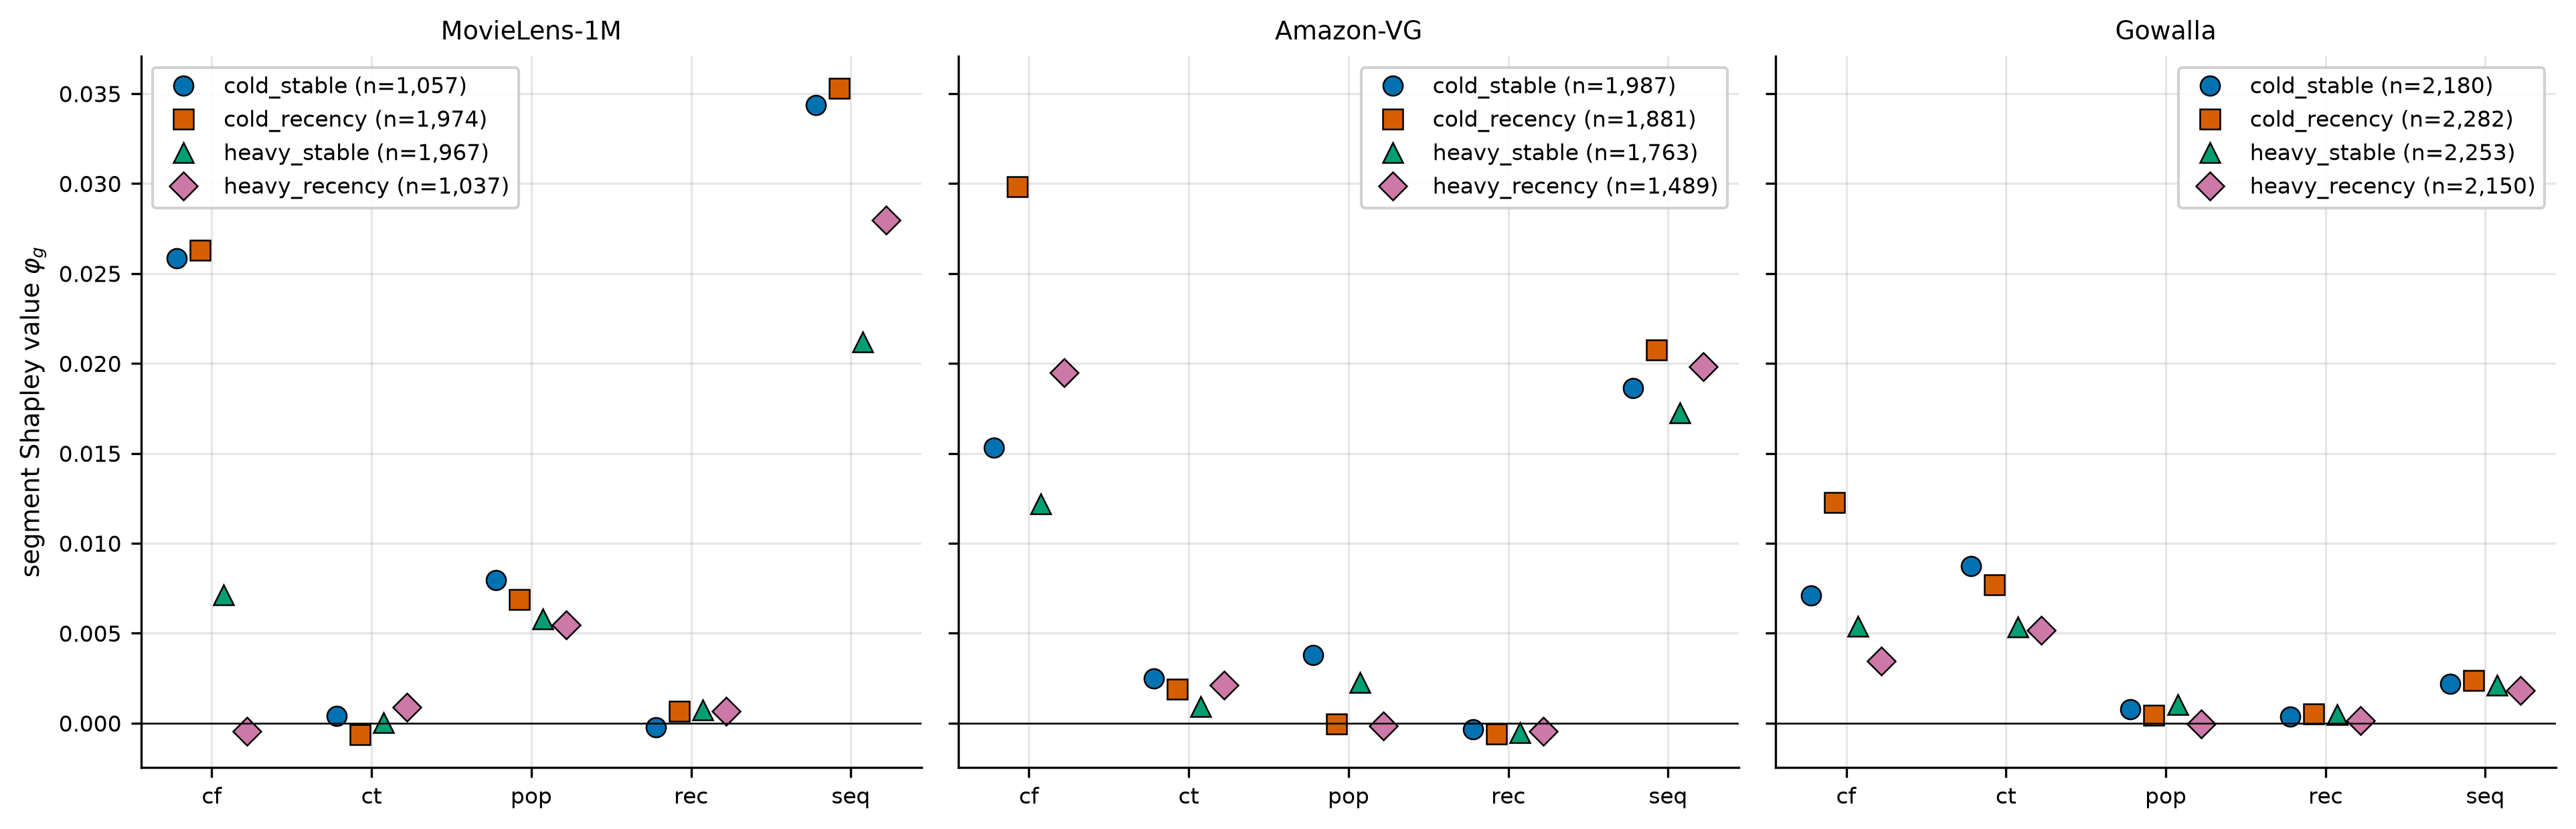
\includegraphics[width=\textwidth]{Fig5.png}
\caption{Descriptive segment-level Shapley values; legends give segment
sizes. No pairwise segment contrast survives within-corpus Holm correction,
so the figure visualises exploratory variation and does not establish
segment-level attribution heterogeneity.}
\label{fig:segments}
\end{figure}

\end{document}
